

%preamble

\documentclass[english]{article}
\usepackage{fullpage}
\usepackage[T1]{fontenc}
\usepackage[latin9]{inputenc}
\setlength{\parskip}{\medskipamount}
\setlength{\parindent}{0pt}

\usepackage{amsmath}
\usepackage{amssymb}
\usepackage{amsthm}
\usepackage{amsfonts}
\usepackage{graphicx}
\usepackage[all,arc,curve,frame]{xy}

\newcommand{\Nat}{\mathbb{N}}
\newcommand{\defeq}{:=}
\newcommand{\vect}[1]{\boldsymbol{#1}}

\renewcommand{\labelenumii}{\arabic{enumi}.\arabic{enumii}.}
\renewcommand{\labelenumiii}{\arabic{enumi}.\arabic{enumii}.\arabic{enumiii}.}
\renewcommand{\labelenumiv}{\arabic{enumi}.\arabic{enumii}.\arabic{enumiii}.\arabic{enumiv}.}



\usepackage{tikz}
\usetikzlibrary{arrows}

\usepackage{float}
\floatstyle{boxed}
\restylefloat{figure}

\usepackage{algorithm}
\usepackage{algorithmic}

\setlength{\abovedisplayskip}{0.5em}
\setlength{\abovedisplayshortskip}{0.5em}
\setlength{\belowdisplayskip}{0.5em}
\setlength{\belowdisplayshortskip}{0.5em}
\setlength{\abovecaptionskip}{0.0em}
\setlength{\belowcaptionskip}{0.0em}

\def\imagetop#1{\vtop{\null\hbox{#1}}}

\newcommand{\xnsysinst}[3]{%
\begin{figure}[H]
\begin{tabular}[c]{l|l}
 \imagetop{#2} &
 \imagetop{\begin{tabular}[c]{@{}l@{}}#3\end{tabular}} \\
\end{tabular}
\caption{Problem instance: \texttt{#1}}
\end{figure}}

\newcommand{\unique}{\exists!}

\begin{document}
\title{
 CS5811 Report:\\
 Search for Self-Stabilizing Protocols
}

\author{~Brandon~Crowley\and~Alex~Klinkhamer\and~Man~Wang}
\maketitle

\newpage
\tableofcontents
\newpage

\section{Project Description}

\subsection{AddConvergence Problem}

Given a network of processes (finite-state machines) and an invariant $I$ over their variables, find a set of actions for the processes which guarantees every computation from any initial global state will eventually reach the invariant (i.e., {\it convergence}).
Additionally, once the system is in an invariant state, it must never leave (i.e., {\it closure}).

For each process $P_i$, network topology defines the variables which $P_i$ owns and which other variables $P_i$ can read.
A process can read and write its own variables and may only read the variables of other processes.
The purpose of a process is to act.
A process can have actions of the form $\mathit{guard} \to \mathit{assignment}$ where $\mathit{guard}$ is a predicate over the readable variables of $P_i$ and $\mathit{assignment}$ is a variable assignment.
\begin{enumerate}
\item If $P_i$ sees a guard is satisfied, it performs the appropriate variable assignment.
 \begin{enumerate}
 \item Note that another process may reassign its variable before $P_i$ can act!
 \end{enumerate}
\item The read/write cycle of an action happens atomically. This is interleaving semantics and we can assume that at most one read/write cycle of an action is happening at any given time.
\item If a process does not have a guard which is satisfied, it does not act.
\item If no two guards can be satisfied at the same time, the process is deterministic.
\end{enumerate}

We can represent actions in the finest possible granularity by considering only local transitions.
For example, if process $P_1$ can read $x_0$ and $x_1$, each spanning $\aset{0,1,2}$, and write $x_1$, then an action 
\[ x_1 = 0 \wedge x_0 = 2 \to x_1 \defeq 1; \]
is a local transition from $(x_1 = 0 \wedge x_0 = 2)$ to $(x_1 = 1 \wedge x_0 = 2)$.
We would not consider an action such as
\[ x_1 = 0 \to x_1 \defeq 1; \]
for $P_1$ because it represents $3$ local transitions:
from $(x_1 = 0 \wedge x_0 = 0)$ to $(x_1 = 1 \wedge x_0 = 0)$,
from $(x_1 = 0 \wedge x_0 = 1)$ to $(x_1 = 1 \wedge x_0 = 1)$,
and from $(x_1 = 0 \wedge x_0 = 2)$ to $(x_1 = 1 \wedge x_0 = 2)$.

\subsection{AddConvergence as a Graph Problem}

We can think of a graph where each vertex corresponds with a global state in the system.
An action is represented by several arcs, each with the same label.
Next mark all global states which satisfy the invariant.

The problem of adding convergence to a system (finding a self-stabilizing protocol) is the same as finding a set of labels for which the set of all arcs with those labels:
\begin{enumerate}
\item Does not include arcs from a vertex marked as invariant to a vertex not marked as invariant.
 \begin{enumerate}
 \item Closure.
 \end{enumerate}
\item Form a path from each vertex not marked as invariant to a vertex marked as invariant.
 \begin{enumerate}
 \item Weak-convergence.
 \end{enumerate}
\item Does not form cycles among the vertices not marked as invariant.
 \begin{enumerate}
 \item Livelock freedom.
 \end{enumerate}
\end{enumerate}

Sometimes no arcs are allowed from any invariant states.

\subsection{Example: Sum-Not-2}

Consider the Sum-Not-2 instance on $3$ processes.
Each process $P_i$ owns a variable $x_i\in\Nat_3$ (where $\Nat_3 = \aset{0,1,2}$).
Processes are in a unidirectional ring meaning each $P_i$ can read its anticlockwise neighbor $P_{i-1}$ (subtraction is modulo $3$).
The invariant is all states where no $x_i + x_{i-1} = 2$, so $I \equiv (\forall i\in\Nat_3: x_i + x_{i-1} \ne 2)$.

Illustrated in the three figures are the problem instance, a stabilizing protocol, and how that protocol appears as a transition graph over the global state space.
\begin{figure}[H]
\begin{tabular}{l|l}
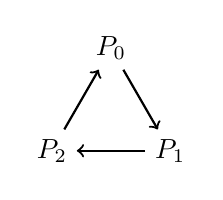
\begin{tikzpicture}[x=1.5cm,y=1.5cm]
\tikzstyle{every node}=[]
\draw
 (0,0)      node (0) {$P_0$}
 ++( -60:1) node (1) {$P_1$}
 ++(-180:1) node (2) {$P_2$}
 ;
\path[->,draw,thick]
(0) edge (1)
(1) edge (2)
(2) edge (0)
;
\end{tikzpicture}
&
\begin{tabular}[b]{@{}l@{}}
For all $i\in\Nat_3$, $P_i$ has privileges:
\\
\begin{centering}
$P_i :
\begin{cases}
 x_i\in\Nat_3 & \mbox{(read-write)} \\
 x_{i-1}\in\Nat_3 & \mbox{(read-only)} \\
\end{cases}$
\end{centering}
\\
Invariant:
$I \equiv (\forall i\in\Nat_3: x_i + x_{i-1} \ne 2)$
\end{tabular}
\\
\end{tabular}
\caption{Sum-Not-2 problem instance.}
\end{figure}

\begin{figure}[H]
\begin{eqnarray*}
   (x_i = 0) \wedge (x_{i-1} = 2) & \to & x_i \defeq 1;
\\ (x_i = 1) \wedge (x_{i-1} = 1) & \to & x_i \defeq 0;
\\ (x_i = 2) \wedge (x_{i-1} = 0) & \to & x_i \defeq 0;
\end{eqnarray*}
\caption{Actions of each $P_i$ in a stabilizing protocol for Sum-Not-2.}
\end{figure}

\begin{figure}[H]
\centering
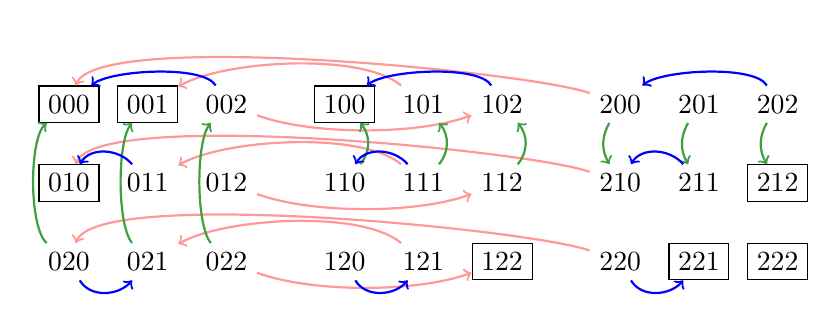
\begin{tikzpicture}[x=1.0cm,y=1.0cm]
\tikzstyle{every node}=[]
\tikzstyle{legit}=[draw]
\def \dx {3.5}
\draw
  (  0, 0) node [legit] (000) {000}
++(\dx, 0) node [legit] (100) {100}
++(\dx, 0) node         (200) {200}
  (  0,-1) node [legit] (010) {010}
++(\dx, 0) node         (110) {110}
++(\dx, 0) node         (210) {210}
  (  0,-2) node         (020) {020}
++(\dx, 0) node         (120) {120}
++(\dx, 0) node         (220) {220}
  (  1, 0) node [legit] (001) {001}
++(\dx, 0) node         (101) {101}
++(\dx, 0) node         (201) {201}
  (  1,-1) node         (011) {011}
++(\dx, 0) node         (111) {111}
++(\dx, 0) node         (211) {211}
  (  1,-2) node         (021) {021}
++(\dx, 0) node         (121) {121}
++(\dx, 0) node [legit] (221) {221}
  (  2, 0) node         (002) {002}
++(\dx, 0) node         (102) {102}
++(\dx, 0) node         (202) {202}
  (  2,-1) node         (012) {012}
++(\dx, 0) node         (112) {112}
++(\dx, 0) node [legit] (212) {212}
  (  2,-2) node         (022) {022}
++(\dx, 0) node [legit] (122) {122}
++(\dx, 0) node [legit] (222) {222}
;
\path[->,draw,thick]
(002) edge [color=red!40,out=- 20,in= 200,looseness=.7] (102)
(012) edge [color=red!40,out=- 20,in= 200,looseness=.7] (112)
(022) edge [color=red!40,out=- 20,in= 200,looseness=.7] (122)
(101) edge [color=red!40,out= 140,in=  30,looseness=.6] (001)
(111) edge [color=red!40,out= 140,in=  30,looseness=.6] (011)
(121) edge [color=red!40,out= 140,in=  30,looseness=.6] (021)
(200) edge [color=red!40,out= 160,in=  70,looseness=.3] (000)
(210) edge [color=red!40,out= 160,in=  70,looseness=.3] (010)
(220) edge [color=red!40,out= 160,in=  70,looseness=.3] (020)

(200) edge [color=green!50!black!75,out=-120,in= 120] (210)
(201) edge [color=green!50!black!75,out=-120,in= 120] (211)
(202) edge [color=green!50!black!75,out=-120,in= 120] (212)
(110) edge [color=green!50!black!75,out=  50,in=- 50] (100)
(111) edge [color=green!50!black!75,out=  50,in=- 50] (101)
(112) edge [color=green!50!black!75,out=  50,in=- 50] (102)
(020) edge [color=green!50!black!75,out= 140,in=-140,looseness=.5] (000)
(021) edge [color=green!50!black!75,out= 130,in=-130,looseness=.5] (001)
(022) edge [color=green!50!black!75,out= 130,in=-130,looseness=.5] (002)

(002) edge [color=blue,out= 120,in=  40,looseness=.5] (000)
(102) edge [color=blue,out= 120,in=  40,looseness=.5] (100)
(202) edge [color=blue,out= 120,in=  40,looseness=.5] (200)
(011) edge [color=blue,out= 130,in=  60] (010)
(111) edge [color=blue,out= 130,in=  60] (110)
(211) edge [color=blue,out= 130,in=  60] (210)
(020) edge [color=blue,out=- 60,in= 230] (021)
(120) edge [color=blue,out=- 60,in= 230] (121)
(220) edge [color=blue,out=- 60,in= 230] (221)
;
\end{tikzpicture}
\caption{Transitions of {\color{red!40} $P_0$}, {\color{green!50!black!75} $P_1$}, {\color{blue} $P_2$}. Legitimate states $x_0x_1x_2$ are boxed.}
\end{figure}

\subsection{Relation to Artificial Intelligence}

The problem of adding convergence is NP-complete in the number of candidate actions (which can be polynomially related to the number of states).

We used techniques from constraint satisfaction problems to get a complete algorithm for AddConvergence.

%* A description of the project and its goals. How does it relate to Artificial Intelligence.

\section{Background}

\subsection{Symbolic Algorithms}

\subsection{Multi-Value Decision Diagram}
As in regular software or any search algorithm, the states could be of large amount and rather complex. Simply listing the states is inefficient and complicates analysis. Here we resort to Multiple-Valued Logic for describing the state of a system, represented by a multi-valued decision diagram (MDD), which is a multi-valued version of the binary decision diagram (BDD).
This allows countermeasures to be formated that address states that share common features. 

MDDs provide a uniform way to represent formulas which evaluate to {\it true} or {\it false} based on variable values (i.e., predicate functions).
We use them because they can also use {\em much less} space than a truth-table.
BDDs and MDDs differ only by the domains of variables. BDDs only allows boolean variables, so they can express the input formulas of the satisfiability problem.
MDDs, on the other hand, allow variables to have finite domains (conventionally represented by natural numbers starting at $0$).
As any integer can be represented by string of bits, MDDs can be implemented using BDDs.

Consider a predicate over three variables $x, y, z$, each with values ranging from $0$ to $4$ (domain size 3). Initially, there are $5^3 = 125$ states in the system. If we specify the state predicate as $x=3$, the number of states for which the predicate returns {\it true} is $25$, since the value of $x$ is totally fixed. We could use an MDD to symbolically represent this set of $25$ states.

Now we have a rough format close to the format representing the protocol states later on. Say there are 3 processes arranged in the bidirectional ring, and each node could read from its two neighbors and write to itself. Actually, with three processes in a bidirectional ring, each process can read all variables, but the small state-space is convenient for this example. We use $m_0$ as the variable of $P_0$. $m'_0$ means the same except the value is the one in the next time step. Similarly, this rule applies to processes $P_1$ and $P_2$. The following predicate represents a transition function for this system:
\begin{eqnarray*}
 & & m_0 = 0 \wedge m'_0 = 0 \wedge m_1 = 0 \wedge m'_1 = 1 \wedge m_2 = 1 \wedge m'_2 = 1 \\
 & \vee & m_0 = 0 \wedge m'_0 = 0 \wedge m_1 = 2 \wedge m'_1 = 1 \wedge m_2 = 1 \wedge m'_2 = 1
\end{eqnarray*}
After checking the values of each process, it is obvious that there are some variables which will change their values as time goes on. The value of $m_1$ can change to $1$ from $0$ when $m_0 = 0 \wedge m_1 = 0 \wedge m_2 = 1$. The value of $m_1$ can also change to $1$ from $2$ when $m_0 = 0 \wedge m_1 = 2 \wedge m_2$. This shows how to represent a transition function with satisfying valuations of unprimed and primed variables.

The following algorithms use set notation, which directly translates to MDD operations.
For example: complement translates to negation, intersection translates to conjunction, and union translates to disjunction.

\subsubsection{Image and Preimage}

The $\vbl{image}(T,S)$ function finds all states which transitions $T$ map from $S$.
\[ \vbl{image}(T,S) = \aset{s_1 \pipe\exists s_0\in S : (s_0,s_1)\in T} \]

The $\vbl{preimage}$ function is the reverse.
It finds all states which are mapped to states in $S$ by transitions $T$.
\[ \vbl{preimage}(T,S) = \aset{s_0 \pipe\exists s_1\in S : (s_0,s_1)\in T} \]

Both $\vbl{image}$ and $\vbl{preimage}$ can be written in terms of MDD operations.

\subsubsection{Weak Convergence}

When checking for weak convergence, we are looking that a path exists from every state outside of the invariant to a state in the invariant.
This algorithm performs backwards reachability from the invariant and returns success if and only if all states can be reached.

\begin{algorithm}[H]{WeakConvergenceCk($T$, $I$)} 
\caption{WeakConvergenceCk} 
\begin{algorithmic}
\STATE $S_0 \defeq I$
\WHILE{$\overline{S_0} \neq \emptyset$}
 \STATE $S_1 \defeq S_0 \cup \vbl{preimage}(T, S_0)$
 \IF{$S_1 = S_0$}
  \RETURN \FALSE
 \ENDIF
 \STATE $S_0 \defeq S_1$
\ENDWHILE
\RETURN \TRUE
\end{algorithmic}
\end{algorithm}

\subsubsection{Cycle Detection}

Check for cycles outside of the invariant by computing the fixed point of the $\vbl{preimage}$ function.
This is the Emerson-Lei algorithm as written in \cite{Fisler:2001:BSC:646485.694446}, but originally from \cite{DBLP:conf/lics/EmersonL86}.
We assume the protocol is closed in the invariant, so we do not need to worry about invariant states being in the preimage.

\begin{algorithm}[H]{CycleCk($T$, $I$)} 
\caption{CycleCk} 
\begin{algorithmic}
\STATE $S_0 \defeq \overline{I}$
\STATE $S_1 \defeq \emptyset$
\REPEAT
 \STATE $S_1 \defeq S_0$
 \STATE $S_0 \defeq S_0 \cap \vbl{preimage}(T,S)$
\UNTIL{$S_0 = S_1$}

\IF{$S_0 = \emptyset$}
 \RETURN \TRUE
\ELSE
 \RETURN \FALSE
\ENDIF
\end{algorithmic}
\end{algorithm}

%\begin{algorithm}{BackwardReachability($T$, $S_1$)}
%\caption{BackwardReachability} 
%\begin{algorithmic}
%\STATE $S_0 \defeq S_1$
%\STATE $L \defeq \vbl{preimage}(T, S_0) - S_0$
%\WHILE{$L \ne \emptyset$}
% \STATE $S_0 \defeq S_0 \cup L$
% \STATE $L \defeq \vbl{preimage}(T, L) - S_0$
%\ENDWHILE
%\RETURN $S_0$
%\end{algorithmic}
%\end{algorithm}

%* Background: related literature and software and algorithms that you imported into your project. Clearly describe, work that you directly used, work you used after modification, and your own contribution.

%* Comparison to similar projects

\section{Examples}
Some examples of stabilizing protocols follow.
We plan to use these (and more) in our experimentation.

We should also try to use reduction to SAT on these problems, but encoding cycle detection in a CNF formula blows up quickly in size.
In the worst case, we require $O(\abs{S_p}^3)$ where $S_p$ is set of all states.
Our tool should outperform the reduction to SAT purely due to its exploding size.

\subsection{Sum-Not-2}

\xnsysinst{sum-not-2}{
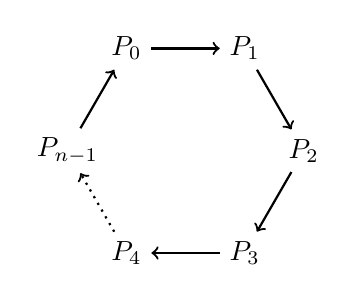
\begin{tikzpicture}[x=1.5cm,y=1.5cm]
\tikzstyle{every node}=[]
 \draw
 (0,0)      node (0) {$P_0$}
 ++(   0:1) node (1) {$P_1$}
 ++( -60:1) node (2) {$P_2$}
 ++(-120:1) node (3) {$P_3$}
 ++(-180:1) node (4) {$P_4$}
 ++(-240:1) node (5) {$P_{n-1}$}
 ;
 \path[->,draw,thick]
 (0) edge (1)
 (1) edge (2)
 (2) edge (3)
 (3) edge (4)
 (5) edge (0)
 ;
 \path[->,draw,thick,dotted]
 (4) edge (5)
 ;
\end{tikzpicture}
}{
For all $i\in\Nat_n$, $P_i$ has privileges:
\\
\begin{centering}
$P_i :
\begin{cases}
 x_i\in\Nat_3 & \mbox{(read-write)} \\
 x_{i-1}\in\Nat_3 & \mbox{(read-only)} \\
\end{cases}$
\end{centering}
\\
Invariant:
$I \equiv (\forall i\in\Nat_n: x_i + x_{i-1} \ne 2)$
}

\subsection{2-Coloring}

\xnsysinst{2-coloring}{
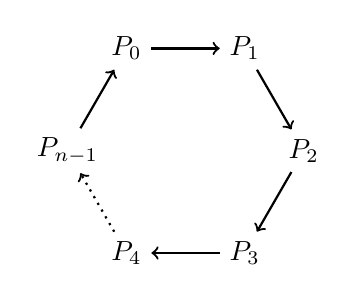
\begin{tikzpicture}[x=1.5cm,y=1.5cm]
\tikzstyle{every node}=[]
 \draw
 (0,0)      node (0) {$P_0$}
 ++(   0:1) node (1) {$P_1$}
 ++( -60:1) node (2) {$P_2$}
 ++(-120:1) node (3) {$P_3$}
 ++(-180:1) node (4) {$P_4$}
 ++(-240:1) node (5) {$P_{n-1}$}
 ;
 \path[->,draw,thick]
 (0) edge (1)
 (1) edge (2)
 (2) edge (3)
 (3) edge (4)
 (5) edge (0)
 ;
 \path[->,draw,thick,dotted]
 (4) edge (5)
 ;
\end{tikzpicture}
}{
For all $i\in\Nat_n$, $P_i$ has privileges:
\\
\begin{centering}
$P_i :
\begin{cases}
 c_i\in\Nat_2 & \mbox{(read-write)} \\
 c_{i-1}\in\Nat_2 & \mbox{(read-only)} \\
\end{cases}$
\end{centering}
\\
Invariant:
\begin{centering}
$I \equiv (\forall i\in\Nat_n: c_{i-1}\ne c_i)$
\end{centering}
}

\subsection{3-Coloring}

\xnsysinst{3-coloring}{
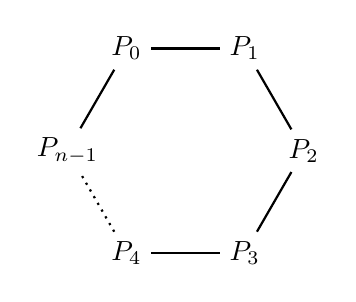
\begin{tikzpicture}[x=1.5cm,y=1.5cm]
\tikzstyle{every node}=[]
 \draw
 (0,0)      node (0) {$P_0$}
 ++(   0:1) node (1) {$P_1$}
 ++( -60:1) node (2) {$P_2$}
 ++(-120:1) node (3) {$P_3$}
 ++(-180:1) node (4) {$P_4$}
 ++(-240:1) node (5) {$P_{n-1}$}
 ;
 \path[draw,thick]
 (0) edge (1)
 (1) edge (2)
 (2) edge (3)
 (3) edge (4)
 (5) edge (0)
 ;
 \path[draw,thick,dotted]
 (4) edge (5)
 ;
\end{tikzpicture}
}{
For all $i\in\Nat_n$, $P_i$ has privileges:
\\
\begin{centering}
$P_i :
\begin{cases}
 c_i\in\Nat_3 & \mbox{(read-write)} \\
 c_{i-1}\in\Nat_3 & \mbox{(read-only)} \\
 c_{i+1}\in\Nat_3 & \mbox{(read-only)} \\
\end{cases}$
\end{centering}
\\
Invariant:
\begin{centering}
$I \equiv (\forall i\in\Nat_n: c_i\ne c_{i-1} \wedge c_i\ne c_{i+1})$
\end{centering}
}

Let each process $P_i$ in a bidirectional ring of $n$ processes have a variable $c_i\in \Nat_3$ (i.e., $c_i\in \{0,1,2\}$) where each of the three values represents a different color, like {\it red}, {\it green}, and {\it blue}.
Since this is a bidirectional ring, any $P_i$ can read its left and right neighbors' variables $c_{i-1}$ and $c_{i+1}$.
$P_i$ can also read and write its own variable $c_i$.

The system is in a legitimate state when no two neighboring processes have the same color.
Formally, the invariant is defined as (with arithmetic modulo $n$):
\[ I \equiv (\forall i\in\Nat_n: c_{i-1}\ne c_i \wedge c_i \ne c_{i+1}) \]

The following action for each $P_i$ can be used for a stabilizing protocol:
\[
 (c_{i-1} = c_i) \vee (c_i = c_{i+1}) \to c_i \defeq \textsc{Other}(c_{i-1}, c_{i+1})
\]
where the \textsc{Other} function returns a color (deterministically, say the minimal-valued one) which is not equal to either of its inputs.

We expect our tool to synthesize actions in their most basic form, as local state transitions.
The above action can be expressed by the following $15$ local state transitions for $P_i$:
\begin{eqnarray*}
 c_{i-1} = 0 \wedge c_i = 0 \wedge c_{i+1} = 0 & \to & c_i \defeq 1 \\
 c_{i-1} = 0 \wedge c_i = 0 \wedge c_{i+1} = 1 & \to & c_i \defeq 2 \\
 c_{i-1} = 1 \wedge c_i = 0 \wedge c_{i+1} = 0 & \to & c_i \defeq 2 \\
 c_{i-1} = 2 \wedge c_i = 0 \wedge c_{i+1} = 0 & \to & c_i \defeq 1 \\
 c_{i-1} = 0 \wedge c_i = 0 \wedge c_{i+1} = 2 & \to & c_i \defeq 1 \\
 c_{i-1} = 1 \wedge c_i = 1 \wedge c_{i+1} = 1 & \to & c_i \defeq 0 \\
 c_{i-1} = 1 \wedge c_i = 1 \wedge c_{i+1} = 0 & \to & c_i \defeq 2 \\
 c_{i-1} = 0 \wedge c_i = 1 \wedge c_{i+1} = 1 & \to & c_i \defeq 2 \\
 c_{i-1} = 1 \wedge c_i = 1 \wedge c_{i+1} = 2 & \to & c_i \defeq 0 \\
 c_{i-1} = 2 \wedge c_i = 1 \wedge c_{i+1} = 1 & \to & c_i \defeq 0 \\
 c_{i-1} = 2 \wedge c_i = 2 \wedge c_{i+1} = 2 & \to & c_i \defeq 0 \\
 c_{i-1} = 2 \wedge c_i = 2 \wedge c_{i+1} = 0 & \to & c_i \defeq 1 \\
 c_{i-1} = 0 \wedge c_i = 2 \wedge c_{i+1} = 2 & \to & c_i \defeq 1 \\
 c_{i-1} = 2 \wedge c_i = 2 \wedge c_{i+1} = 1 & \to & c_i \defeq 0 \\
 c_{i-1} = 1 \wedge c_i = 2 \wedge c_{i+1} = 2 & \to & c_i \defeq 0
\end{eqnarray*}

\subsection{Maximal Matching}

\xnsysinst{matching}{
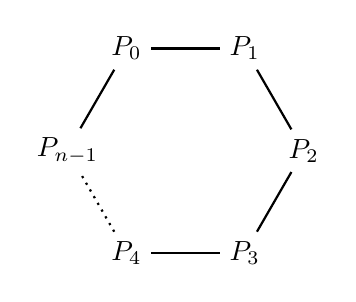
\begin{tikzpicture}[x=1.5cm,y=1.5cm]
 \tikzstyle{every node}=[]
 \draw
 (0,0)      node (0) {$P_0$}
 ++(   0:1) node (1) {$P_1$}
 ++( -60:1) node (2) {$P_2$}
 ++(-120:1) node (3) {$P_3$}
 ++(-180:1) node (4) {$P_4$}
 ++(-240:1) node (5) {$P_{n-1}$}
 ;
 \path[draw,thick]
 (0) edge (1)
 (1) edge (2)
 (2) edge (3)
 (3) edge (4)
 (5) edge (0)
 ;
 \path[draw,thick,dotted]
 (4) edge (5)
 ;
\end{tikzpicture}
}{
For all $i\in\Nat_n$, $P_i$ has privileges:
\\
\begin{centering}
$P_i :
\begin{cases}
 m_i\in\Nat_3 & \mbox{(read-write)} \\
 m_{i-1}\in\Nat_3 & \mbox{(read-only)} \\
 m_{i+1}\in\Nat_3 & \mbox{(read-only)} \\
\end{cases}$
\end{centering}
\\
Invariant:
\\
\begin{centering}
$\begin{array}{rcl}
 I \equiv \forall i\in\Nat_n: & & (m_{i-1} = 2 \wedge m_i = 1)
\\ & \vee  & (m_{i-1} = 1 \wedge m_i = 0 \wedge m_{i+1} = 2)
\\ & \vee  & (m_i = 2 \wedge m_{i+1} = 1)
\end{array}$
\end{centering}
}

Let each process $P_i$ in a bidirectional ring of $n$ processes have a variable $m_i\in \Nat_3$ (i.e., $m_i\in \{0,1,2\}$) where each of the three values represents a different direction, like {\it self} ($m_i=0$), {\it left} ($m_i=1$), and {\it right} ($m_i=2$).
Since this is a bidirectional ring, any $P_i$ can read its left and right neighbors' variables $m_{i-1}$ and $m_{i+1}$.
$P_i$ can also read and write its own variable $m_i$.

The system is in a legitimate state when neighbors pair up by pointing at each other.
If both neighbors are pointing away, a process can point at itself.
Formally, the invariant is defined as (with arithmetic modulo $n$):
\begin{eqnarray*}
 I \equiv \forall i\in\Nat_n: & & (m_{i-1} = 2 \wedge m_i = 1)
                    \\ & \vee  & (m_{i-1} = 1 \wedge m_i = 0 \wedge m_{i+1} = 2)
                    \\ & \vee  & (m_i = 2 \wedge m_{i+1} = 1)
\end{eqnarray*}


\subsection{Dijkstra's Token Ring \cite{dij}}

\xnsysinst{dijkstra-tr}{
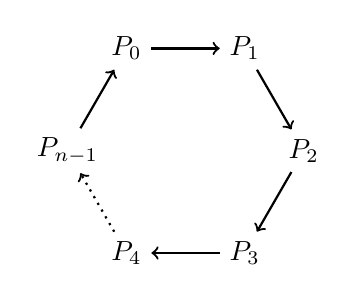
\begin{tikzpicture}[x=1.5cm,y=1.5cm]
 \tikzstyle{every node}=[]
 \draw
 (0,0)      node (0) {$P_0$}
 ++(   0:1) node (1) {$P_1$}
 ++( -60:1) node (2) {$P_2$}
 ++(-120:1) node (3) {$P_3$}
 ++(-180:1) node (4) {$P_4$}
 ++(-240:1) node (5) {$P_{n-1}$}
 ;
 \path[->,draw,thick]
 (0) edge (1)
 (1) edge (2)
 (2) edge (3)
 (3) edge (4)
 (5) edge (0)
 ;
 \path[->,draw,thick,dotted]
 (4) edge (5)
 ;
\end{tikzpicture}
}{
For all $i\in\Nat_n$, $P_i$ has privileges:
\\
\begin{centering}
$P_i :
\begin{cases}
 x_i\in\Nat_{n+1} & \mbox{(read-write)} \\
 x_{i-1}\in\Nat_{n+1} & \mbox{(read-only)} \\
\end{cases}$
\end{centering}
\\
Invariant:
\\
\begin{centering}
$I\equiv (\mbox{$\unique i\in\Nat_n$: $\mathtt{token?}(i)$})$
\end{centering}
\\
\begin{centering}
$\mathtt{token?}(i) = \begin{cases}
   x_i = x_{i-1} & i = 0
\\ x_i \ne x_{i-1} & i \ne 0
\end{cases}$
\end{centering}
}

Let us consider the original token ring protocol Dijkstra used when introducing the concept of self-stabilization \cite{dij}.
A token ring is used to give one process out of many an exclusive right, also known as distributed mutual exclusion.
Below is a ring of $n=6$ finite-state machines (processes).

Each process $P_i$ holds a variable $x_i$ which ranges from $0$ to $n$ ($x_i\in\Nat_{n+1}$).
Each $P_i$ can read and write $x_i$ and can read $x_{i-1}$ (where subtraction is modulo $n$).
Note that each process can only read its left neighbor, so we call this ring {\em unidirectional}.

$P_0$ is said to have a token when it sees $x_{n-1} = x_0$.
Any other $P_i$ has a token when $x_{i-1} \neq x_i$.

A state is legitimate when exactly one process has the token.

\[
\begin{array}{rrcl}
 P_0: & x_{5} = x_0 & \to & x_0 \defeq x_0 + 1 \mod (n+1)
\\ P_{i>0}: & x_{i-1} \neq x_i & \to & x_i \defeq x_{i-1}
\end{array}
\]

\subsection{2-Bit Token ``Spring'' \cite{dij}}

\xnsysinst{2-bit-tr}{
\begin{tikzpicture}[x=1.5cm,y=1.5cm]
  \tikzstyle{every node}=[]
  \draw
  (0,0)      node (0) {$P_0$}
  ++( -30:1) node (1) {$P_1$}
  ++( -90:1) node (2) {$P_2$}
  ++(-150:1) node (3) {$P_3$}
  ++(-210:1) node (4) {$P_4$}
  ++(-270:1) node (5) {$P_{n-1}$}
  ;
  \path[draw,thick]
  (0) edge (1)
  (1) edge (2)
  (2) edge (3)
  (3) edge (4);
  \path[draw,thick,dotted]
  (4) edge (5);
\end{tikzpicture}
}{
For all $i\in\Nat_n$, $P_i$ has privileges:
\\
\begin{centering}
$P_i :
\begin{cases}
   x_i\in\Nat_2 & \mbox{(read-write)}
\\ \vbl{up}_i\in\Nat_2 & \mbox{(read-write)}
\\ x_{i-1}\in\Nat_2 & \mbox{(read-only) when $i>0$}
\\ x_{i+1}\in\Nat_2 & \mbox{(read-only) when $i<n-1$}
\\ \vbl{up}_{i+1}\in\Nat_2 & \mbox{(read-only) when $i<n-1$}
\end{cases}$
\end{centering}
\\
Invariant:
\\
\begin{centering}
$I\equiv (\mbox{$\unique i\in\Nat_n$: $\mathtt{token?}(i)$}) \wedge \vbl{up}_0 = 1 \wedge \vbl{up_1} = 0$
\end{centering}
\\
\begin{centering}
$\mathtt{token?}(i) = \begin{cases}
   x_i = x_{i+1} \wedge \vbl{up}_{i+1} = 0 & i = 0
\\ x_i = x_{i+1} \wedge \vbl{up}_i = 1 \wedge \vbl{up}_{i+1} = 0 & 0<i<n-1
\\ x_i \ne x_{i-1} & 0 < i
\end{cases}$
\end{centering}
}

\subsection{3-Bit Token Rring \cite{Gouda:3bitTR}}

\xnsysinst{3-bit-tr}{
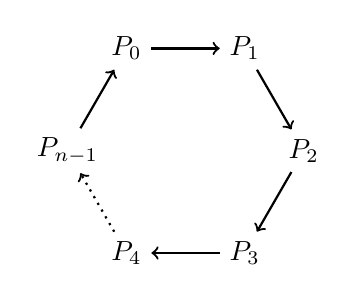
\begin{tikzpicture}[x=1.5cm,y=1.5cm]
 \tikzstyle{every node}=[]
 \draw
 (0,0)      node (0) {$P_0$}
 ++(   0:1) node (1) {$P_1$}
 ++( -60:1) node (2) {$P_2$}
 ++(-120:1) node (3) {$P_3$}
 ++(-180:1) node (4) {$P_4$}
 ++(-240:1) node (5) {$P_{n-1}$}
 ;
 \path[->,draw,thick]
 (0) edge (1)
 (1) edge (2)
 (2) edge (3)
 (3) edge (4)
 (5) edge (0)
 ;
 \path[->,draw,thick,dotted]
 (4) edge (5)
 ;
\end{tikzpicture}
}{
For all $i\in\Nat_n$, $P_i$ has privileges:
\\
\begin{centering}
$P_i :
\begin{cases}
 e_i\in\Nat_2 & \mbox{(read-write)}
\\ t_i\in\Nat_2 & \mbox{(read-write)}
\\ \vbl{ready}_i\in\Nat_2 & \mbox{(read-write)}
\\ e_{i-1}\in\Nat_2 & \mbox{(read-only)}
\\ t_{i-1}\in\Nat_2 & \mbox{(read-only)}
\end{cases}$
\end{centering}
\\
Invariant:
\\
\begin{centering}
$I\equiv (\mbox{$\unique i\in\Nat_n$: $\mathtt{t\_token?}(i)$})\wedge(\exists i\in\Nat_n: \mathtt{e\_token?}(i))$
\end{centering}
\\
\begin{centering}
$\mathtt{e\_token?}(i) = \begin{cases}
   e_i = e_{i-1} & i = 0
\\ e_i \ne e_{i-1} & i \ne 0
\end{cases}$
\end{centering}
\\
\begin{centering}
$\mathtt{t\_token?}(i) = \begin{cases}
   t_i = t_{i-1} & i = 0
\\ t_i \ne t_{i-1} & i \ne 0
\end{cases}$
\end{centering}
}
\newpage
\section{Experiments}
%* Experiments: Clearly and in detail describe the experimental setup. Use a "storyboard" like approach if possible. Give all the information so that
% someone who reads the report can replicate your experiments. Explain and discuss the experimental results. How were the problems selected? Did you
% use problems with varying complexity and test the boundaries of the system?
For all of the following experiments, results were gather for an increasing number of processors until the runtime crossed a threshhold of 5 minutes.
Timing was gathered using the "time" command in bash.  The number of states is given as a reference from knowledge of the problem, not as an
experimental result.
\begin{center}
2-coloring \\
\begin{tabular}{|c|c|c|c|c|}
\hline
 Processes & Time (sec) & Solution Size & Backtrack Depth & States \\
\hline
 2 & .009 & 2 & 2 & $2^{2}$             \\
 4 & .01 & 6 & 6 & $2^{4}$              \\
 6 & .015 & 10 & 10 & $2^{6}$           \\
 8 & .047 & 14 & 14 & $2^{8}$           \\
 10 & .15 & 18 & 18 & $2^{10}$          \\
 12 & .486 & 22 & 22 & $2^{12}$         \\
 14 & 1.346 & 26 & 26 & $2^{14}$        \\
 16 & 3.595 & 30 & 30 & $2^{16}$        \\
 18 & 10.547 & 34 & 34 & $2^{18}$       \\
 20 & 34.282 & 38 & 38 & $2^{20}$       \\
\hline
\end{tabular}
\end{center}

The 2-coloring experiment was run for even numbered processes on the range of [2..20].  This domain was chosen because an even number of processes
cannot stabilize in a 2-coloring problem.  This is a fairly uncomplicated problem, so the results aren't all that unusual.  The solution size and depth
increase linearly at a rate of 4.  The timing increases roughly linearly at a rate of 3 when the number of processors is 6 and greater.  This serves
mostly as a baseline problem for the stabilizer.

\begin{center}
3-coloring \\
\begin{tabular}{|c|c|c|c|c|}
\hline
 Processes & Time (sec) & Solution Size & Backtrack Depth & States \\
\hline
 2 & .003 & 3 & 3 & $3^{2}$           \\
 3 & .039 & 21 & 21 & $3^{3}$         \\
 4 & .105 & 30 & 30 & $3^{4}$          \\
 5 & .63 & 33 & 32 & $3^{5}$          \\
 6 & 1.728 & 39 & 38 & $3^{6}$        \\
 7 & 7.726 & 45 & 44 & $3^{7}$        \\
 8 & 15.887 & 51 & 50 & $3^{8}$       \\
 9 & 74.22 & 59 & 58 & $3^{9}$        \\
 10 & 134.946 & 65 & 64 & $3^{10}$    \\
\hline
\end{tabular}
\end{center}

The 3-coloring problem turned out to be a bit more interesting.  It was run for processors numbering [2..10].  The rates of increase area all variable
for this experiment.  For the lower processor numbers, timing saw increases of up to 10 times, and the solution size and backtrack depths saw increases
of up to 7 times.  You can also see that the solution size and backtrack depth differ in this problem.  This means that the algorithm was able to infer
an action during forward checking, without actually exploring it.  This prevents the program from having to explore more paths, reducing the overall
runtime.  The increases in runtime also correlate roughly with the increases in solution size and backtrack depth.  Since there is not a whole lot
of backtracking that needs to be done for a 3-coloring problem, this makes sense.  If there is the increase in runtime is disproportionate to the
increases in solution size and backtrack depth, it most likely means that backtracking had to occur, causing more work for a smaller or less deep
solution.

\begin{center}
Sum Not 2 \\
\begin{tabular}{|c|c|c|c|c|}
\hline
 Processes & Time (sec) & Solution Size & Backtrack Depth & States \\
\hline
 2 & .002 & 3 & 3 & $3^{2}$               \\
 3 & .006 & 9 & 9 & $3^{3}$               \\
 4 & .014 & 12 & 12 & $3^{4}$             \\
 5 & .047 & 15 & 15 & $3^{5}$             \\
 6 & .15 & 18 & 18 & $3^{6}$              \\
 7 & .361 & 21 & 21 & $3^{7}$              \\
 8 & .743 & 24 & 24 & $3^{8}$             \\
 9 & 1.381 & 27 & 27 & $3^{9}$            \\
 10 & 2.463 & 30 & 30 & $3^{10}$          \\
 11 & 4.292 & 33 & 33 & $3^{11}$          \\
 12 & 7.098 & 36 & 36 & $3^{12}$          \\
 13 & 11.79 & 39 & 39 & $3^{13}$          \\
 14 & 19.002 & 42 & 42 & $3^{14}$         \\
 15 & 30.676 & 45 & 45 & $3^{15}$         \\
 16 & 49.034 & 48 & 48 & $3^{16}$         \\
 17 & 72.74 & 51 & 51 & $3^{17}$          \\
 18 & 106.68 & 54 & 54 & $3^{18}$          \\
 19 & 152.64 & 57 & 57 & $3^{19}$         \\
 20 & 210.548 & 60 & 60 & $3^{20}$        \\
\hline
\end{tabular}
\end{center}
 
\begin{center}
Dijsktra's Token Ring \\
\begin{tabular}{|c|c|c|c|c|}
\hline
 Processes & Time (sec) & Solution Size & Backtrack Depth & States \\
\hline
 3 & .023 & 28 & 8 & $4^{3}$         \\
 4 & 7.165 & 65 & 13 & $5^{4}$          \\
\hline
\end{tabular}
\end{center}

\begin{center}
2-bit Token Spring \\
\begin{tabular}{|c|c|c|c|c|}
\hline
 Processes & Time (sec) & Solution Size & Backtrack Depth & States \\
\hline         
 2 & .01 & 14 & 9 & $4^{2}$         \\
 3 & .055 & 21 & 13 & $4^{3}$       \\
 4 & 1.019 & 26 & 13 & $4^{4}$      \\
 5 & 5.402 & 31 & 13 & $4^{5}$      \\
 6 & 17.789 & 37 & 14 & $4^{6}$     \\
 7 & 48.017 & 43 & 15 & $4^{7}$     \\
 8 & 113.130 & 49 & 16 & $4^{8}$    \\
 9 & 250.614 & 55 & 17 & $4^{9}$    \\
\hline
\end{tabular}
\end{center}

\begin{center}
3-bit Token Ring \\
\begin{tabular}{|c|c|c|c|c|}
\hline
 Processes & Time (sec) & Solution Size & Backtrack Depth & States \\
\hline         
 3 & .631 & 53 & 52 & $8^{3}$       \\
 4 & 5.862 & 70 & 68 & $8^{4}$      \\
 5 & 64.304 & 97 & 95 & $8^{5}$      \\
\hline
\end{tabular}
\end{center}

\begin{center}
Matching-Heavy Greedy Heuristic \\
\begin{tabular}{|c|c|c|c|c|}
\hline
 Processes & Time (sec) & Solution Size & Backtrack Depth & States \\
\hline         
 2 & .047 & 7 & 6 & $3^{2}$        \\
 3 & .062 & 24 & 24 & $3^{3}$       \\
 4 & .594 & 38 & 35 & $3^{4}$      \\
 5 & 1.167 & 45 & 41 & $3^{5}$      \\
 6 & 6.811 & 61 & 52 & $3^{6}$     \\
 7 & 16.042 & 69 & 60 & $3^{7}$    \\
 8 & 53.214 & 75 & 66 & $3^{8}$    \\
\hline
\end{tabular}

Matching-Light Greedy Heuristic \\
\begin{tabular}{|c|c|c|c|c|}
\hline
 Processes & Time (sec) & Solution Size & Backtrack Depth & States \\
\hline         
 2 & .006 & 7 & 6 & $3^{2}$        \\
 3 & .105 & 24 & 24 & $3^{3}$       \\
 4 & .69 & 36 & 34 & $3^{4}$      \\
 5 & 2.291 & 46 & 40 & $3^{5}$      \\
 6 & 6.444 & 60 & 52 & $3^{6}$     \\
 7 & 17.944 & 61 & 59 & $3^{7}$    \\
 8 & 64.787 & 73 & 65 & $3^{8}$    \\
\hline
\end{tabular}
\end{center}

\section{Instructions to Run Code}
%* Full commented code with instructions to run it as is and with different parameters.
\subsection{Running the code}
The program could be executed in terminal using the following command:

\[
  ./bin/protocon <problem> <numprocs>
\]

where

$\textbf{\emph{<problem>}}$ is one of:

"3-coloring", "2-coloring", "matching", "sum-not-2", "dijkstra-tr", "3-bit-tr", "2-bit-tr"

$\textbf{\emph{<numprocs>}}$ is number of processes

\subsection{Outputs}
In the output, there are two sections. The first section shows the type of ring and the steps the program took. And the second section is a summery of the actions each process has taken.

In the first secion,

$\textbf{\emph{(lvl\ n)}}$ means that the output is generated at the level $n$ of recursion. At least $n$ actions will be chosen at this point.

$\textbf{\emph{(sz\ n)}}$ means that there are actually $n$ actions chosen. It can be larger than the recursion level if the actions are included based on forward-checking.

$\textbf{\emph{(rem\ n)}}$ means that there are $n$ remaining candidate actions at this point. The part printed after is the action being chosen, which is indicated in $\textbf{\emph{(sz\ m)}}$ before. 

$\textbf{\emph{(lvl\ x) (mcv\ y) (mcv-sz\ z)}}$ is printed when making the decision to pick the next action (applying the MCV heuristic). This one is at level $x$, where the most constrained deadlock(s) have only $y$ different candidate actions that resolve them, but there are many sets of deadlocks which may only be resolved by $y$ different candidate actions. In total, $z$ candidate actions can resolve one of these most-constrained deadlocks.

In the second section, the success or failure of finding a solution will be shown first. If the solution is successfully found. It is going to be represented in a series of actions listed in the order of process indices. The actions are presented in the form: 
\[
process:\ state\ before\ action\ ->\ action\ executed
\]
where $"state\ before\ action"$ are only the states that trigger the following action. 

\section{Task Distribution}
%* How were the tasks distributed among the group members? How long did it take for tasks to complete?

\begin{center}
\begin{tabular}{|c||c|c|c|}
\hline
 Task & Estimate & People & Status \\
\hline
 BDD & 1 week, 2 people & all & done \\
 Topology & 1 week, 3 people & all & done \\
 Input File & 3 days, 3 people & all & N/A \\
 Weak Stabilization Check & 2 days, 1 person & Mandy & done \\
 Cycle Check & 1 week, 1 person & Alex & done \\
 Backtracking Algorithm & 4 days, 2 people & Brandon \& Mandy & done \\
 Output File & 1 day, 1 person &  Brandon & N/A \\
 Output Model & 1 day, 1 person & Alex & done \\
 Forward Checking & 2 days, 3 people & all & done \\
 Most-Constrained Variable & 1 week, 3 people & all & done \\
 AC-3 & 1 week, 3 people & all & done, removed \\
 Examples and Comparison & 2 weeks, 3 people & all & done \\
\hline
\end{tabular}
\end{center}

\section{Contributions and Accomplishments}
%* Contributions and accomplishments. Were you able to accomplish the minimal set of goals identified in your proposal? What else was accomplished? Make sure to define accomplishments specifically, supplementing phrases such as "better" or "improved" by numeric data.

This work gives some insight on why polynomial-time heuristic methods such as \cite{ipdpsEbnenasir11} succeed.
We were able to avoid backtracking in many cases by simply choosing actions in the proper order, combined with forward-checking.

\section{Lessons Learned}

We learned that it is simple to collaborate on code and documentation in version control.

\section{Future Work}

This work gives some insight on why polynomial-time heuristic methods such as \cite{ipdpsEbnenasir11} succeed.
We were able to avoid backtracking in many cases by simply choosing actions in the proper order, combined with forward-checking.

\section{Project Comments and Suggestions}
%* Any comments and suggestions of the project component of CS5811 will be appreciated.



%{\it Formulate the search problem: states, actions, goals.}


\bibliographystyle{plain}
\bibliography{bibliography}

\end{document}

